\slide{Tratamento dos Dados}{
    \begin{itemize}
        \item Inicialmente, os dados possuíam algumas colunas inconsistentes, ou não que eram necessárias para o problema e, por isso, foram removidas.
        \begin{table}[htbp]
            \begin{tabular}{ccccccc}
            \toprule
            \multicolumn{1}{l}{\textbf{Id Equi.}} & \multicolumn{1}{l}{\textbf{A/M/D}} & \multicolumn{1}{l}{\textbf{\textcolor{red}{Hora}}} & \multicolumn{1}{l}{\textbf{\textcolor{red}{Faixa}}} & \multicolumn{1}{l}{\textbf{km/h}} & \multicolumn{1}{l}{\textbf{\textcolor{red}{km/h Max}}} & \multicolumn{1}{l}{\textbf{\textcolor{red}{Tam.}}} \\ 
            \bottomrule
            \end{tabular}
            \caption{Colunas removidas destacadas em vermelho}
        \end{table}
        \item RSI128
    \end{itemize}
}

\slide{Transformação dos Dados}{
    A coluna \textit{Data} teve o seu formato alterado para melhorar o treinamento dos modelos e evitar falsas suposições por parte dos modelos. Para realizar a transformação utilizou-se de \textit{One Hot Enconding}. Separando assim em 7 colunas booleanas.
    
    \vspace{25pt}
    
    \resizebox{\columnwidth}{!}{
        \begin{table}[H]
            \begin{tabular}{ccccccc}
            \toprule
            \textbf{Domingo} & \textbf{Segunda} & \textbf{Terça} & \textbf{Quarta} & \textbf{Quinta} & \textbf{Sexta} & \textbf{Sábado} \\
            \midrule
            |1|0|0|0|0|0|0| & |0|1|0|0|0|0|0| & |0|0|1|0|0|0|0| & |0|0|0|1|0|0|0| & |0|0|0|0|1|0|0| & |0|0|0|0|0|1|0| & |0|0|0|0|0|0|1| \\
            \bottomrule
            \end{tabular}
        \end{table}
    }
}

\slide{Sazonalidade dos Dados}{
 \begin{figure}[htbp]
        \centering
        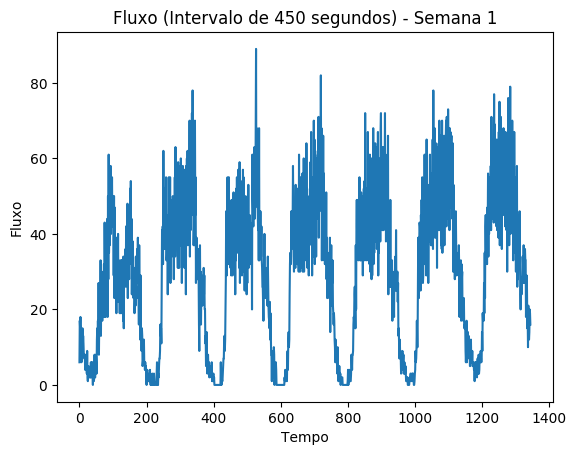
\includegraphics[scale=0.55]{monography/img/flows/flow_450_week_01.png}
        \caption{Exemplo de fluxo semanal}
    \end{figure}
}

\slide{Acumulação dos Dados}{
    Com todas as colunas no formato adequado, o conjunto de registro de veículos foi transformado em um conjunto de acumulação de fluxo de veículos. Foram geradas as seguintes colunas:

    \begin{itemize}
         \item \textbf{Fluxo}: Quantidade de veículos em um determinado intervalo de tempo;
        \item \textbf{Velocidade Média}: Velocidade média dos veículos nesse mesmo intervalo de tempo;
        \item \textbf{Densidade}: Fluxo dividido pela Velocidade média dos veículos, em um intervalo de tempo;
    \end{itemize}
}

\slide{Dados Após o Tratamento Completo}{
   \begin{table}[H]
    \begin{tabular}{cccccccccc}
    \toprule
    \multicolumn{1}{l}{\textbf{Fluxo}} & \multicolumn{1}{l}{\textbf{Densidade}} & \multicolumn{1}{l}{\textbf{Velocidade Média}} & \multicolumn{1}{l}{\textbf{D}} &
    \multicolumn{1}{l}{\textbf{S}} & \multicolumn{1}{l}{\textbf{T}} & \multicolumn{1}{l}{\textbf{Q}} & \multicolumn{1}{l}{\textbf{Q}} &
    \multicolumn{1}{l}{\textbf{S}} &
    \multicolumn{1}{l}{\textbf{S}} \\
    \midrule
    6 & 0.26 & 23.50 & 0 & 0 & 0 & 0 & 0 & 0 & 1 \\
    \midrule
    17 & 0.58 & 29.23 & 0 & 0 & 0 & 0 & 0 & 1 & 0 \\
    \midrule
    15 & 0.62 & 24.93 & 0 & 0 & 0 & 0 & 1 & 0 & 0 \\
    \midrule
    18 & 0.66 & 27.50 & 0 & 0 & 0 & 1 & 0 & 0 & 0 \\
    \bottomrule
    \end{tabular}
        \caption{Exemplo das colunas do conjunto de dados após a transformação (7.5 minutos de fluxo)}
\end{table}
}

\slide{Conjuntos de Treino e Teste}{
    \begin{itemize}
        \item Dois conjunto de treinamento:
            \begin{itemize}
                \item A: 1 atributo, o fluxo;
                \item B: todos os atributos mostrados;
            \end{itemize}
        \item Utilização de uma parte do passado para prever o futuro;
    \end{itemize}
  
}

\slide{Out-of-Sample-Testing}{
 
 \begin{itemize}
     \item Cross-Validation não pode ser utilizado;
     \item Out-of-Sample-Testing;
     \item Origem deslizante;
 \end{itemize}
 
 }

\slide{Out-of-Sample Testing}{
    \begin{figure}[htbp]
        \centering
        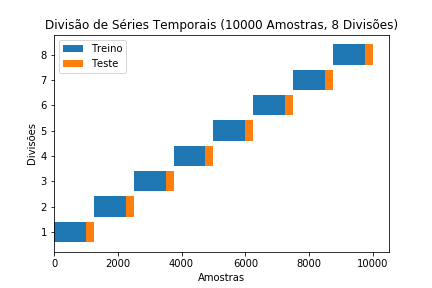
\includegraphics[scale=0.65]{monography/img/methods/blocking_cv.png}
    \end{figure}
}

\slide{Métricas de Avaliação}{
    \begin{equation}
        \label{eq:mae}
        MAE = \frac{1}{n} \times \sum_{i=1}^{n} \quad \abs{y_i - \hat{y_i}}
    \end{equation}

    \begin{equation}
        \label{eq:rmse}
        RMSE = \sqrt{ \frac{1}{n} \times \sum_{i=1}^{n} \quad (y_i - \hat{y_i}) ^ 2}
    \end{equation}
}

\slide{Métricas de Avaliação}{
    \begin{equation}
        f(a, b, k) =
        \begin{cases}
          0, & \text{if}\ (a - k) \times (b - k) \textless 0 \\
          1, & \text{caso contrário}
        \end{cases}
    \end{equation}
    
    \begin{equation}
        \alpha = \frac{100\%}{n} \times \sum_{i=1}^{n} f(y_i, \hat{y_i}, x_{i, m_{fluxo}})
    \end{equation}
}

\slide{Bases de Comparação}{
    \begin{itemize}
        \item \textbf{Média Móvel}: Média dos fluxos da entrada;
        \item \textbf{Naive}: retorna o fluxo mais recente da entrada;
    \end{itemize}
}

\slide{Escolha dos Parâmetros}{
    \begin{itemize}
        \item \textbf{Número de divisões do conjunto de dados} (\textit{Blocking}): 1, 2, 4, 8 divisões;
        \item \textbf{Passado Visível}: 60, 120, 240 e 480 minutos;
        \item \textbf{Tamanho do Intervalo para cálculo do fluxo}: 150, 300, 450 segundos;
    \end{itemize}
}

\slide{Treino}{
    \begin{algorithm}[H]
        \begin{algorithmic}[H]
            \REQUIRE $X$, $Y$, $k$ (número de divisões)
            \ENSURE $[\hat{y_0}, ..., \hat{y_k}]$
            \STATE $\hat{Y} \leftarrow [] $
            \FOR{$(X_{train}, X_{test}, Y_{train}, Y_{test})$ $\in$ $divisaoBlocos(X, Y, k)$} 
                \STATE $modelo \leftarrow geraModelo()$
                \STATE $modelo \leftarrow treinaModelo(modelo, X_{train}, Y_{train})$ 
                \STATE $\hat{y} \leftarrow predizModelo(modelo, X_{test}) $
                \STATE $\hat{Y} \leftarrow \hat{Y} + \hat{y}$
            \ENDFOR
            \RETURN $\hat{Y}$
        \end{algorithmic}
    \end{algorithm}
}

\slide{Escolha dos Hiper-parâmetros}{
    \textbf{Específicos de Aprendizagem Profunda:}
    \begin{itemize}
        \item \textbf{Taxa de Aprendizado}: 0.001, 0.004, 0.016 e 0.064;
        \item \textbf{Número de Células da Rede}: 50, 75, 100, 125 células;
    \end{itemize}
    \textbf{Específicos de RF:}
    \begin{itemize}
        \item \textbf{Quantidade de Estimadores}: 50, 100, 200, 400, 800 estimadores;
        \item \textbf{Altura Máxima}: 8, 16, 32, 64 e sem limitações no tamanho;
    \end{itemize}
    \textbf{Específicos de SVM:}
    \begin{itemize}
        \item \textbf{C}: 1, 10, 100 e 1000;
        \item \textbf{\(\gamma\)}: \(10^{-2}\), \(10^{0.\overline{3}}\), \(10^{0.\overline{6}}\), \( 10^{2}\), e o padrão da biblioteca; 
    \end{itemize}
}

\slide{Treino com \textit{Tuning}}{
    \begin{algorithm}[H]
        \begin{algorithmic}[H]
            \REQUIRE $X$, $Y$, $k$ (número de divisões)
            \ENSURE $[\hat{y_0}, ..., \hat{y_k}]$
            \STATE $\hat{Y} \leftarrow [] $ 
            \FOR{$(X_{train}, X_{test}, Y_{train}, Y_{test})$ $\in$ $divisaoBlocos(X, Y, k)$} 
                \STATE $hp \leftarrow pegarHiperParametros()$
                \STATE $dados \leftarrow divisaoBlocos(X_{train}, Y_{train}, 1)$
                \STATE $modelo \leftarrow escolheMelhorModelo(geraModelo, hp, dados)$
                \STATE $modelo \leftarrow treinaModelo(modelo, X_{train}, Y_{train})$ 
                \STATE $\hat{y} \leftarrow predizModelo(modelo, X_{test}) $
                \STATE $\hat{Y} \leftarrow \hat{Y} + \hat{y}$
            \ENDFOR
        \RETURN $\hat{Y}$
        \end{algorithmic}
    \end{algorithm}
}